\documentclass{article}
\usepackage[utf8]{inputenc}   
\usepackage[T1]{fontenc}      
\usepackage{graphicx}         
\usepackage{geometry} 
\usepackage{url}
\usepackage{setspace}
\usepackage{caption}
\usepackage{booktabs}
\usepackage{titlesec}
\usepackage{amsmath}
\usepackage[backend=biber, style=authoryear, maxcitenames=2, mincitenames=1]{biblatex}
\addbibresource{biblio.bib}
\usepackage{hyperref}
\renewcommand{\figurename}{\textsc{Figure}}
\captionsetup[figure]{labelsep=period}
\captionsetup[table]{labelfont={sc},labelsep=period,name=Table}
\geometry{a4paper, margin=2.5cm}

\begin{document}
\setlength{\parindent}{0pt}
\setlength{\bibitemsep}{0.5\baselineskip}

\begin{flushleft}
\text{Eyquem Martin-Skutnik}
\end{flushleft}

\vspace{8pt}

\begin{center}
    \large\textbf{Big Data and Business Analytics} \\[1pt]
    \large\textit{Final Project} \\[8pt]
\end{center}

\vspace{4pt}

\begin{setstretch}{1.34}
\section{Introduction}

This report addresses the stock price movement prediction task by combining textual sentiment data with traditional financial features within a unified Bayesian forecasting framework. Using 3 million tweets and supplementary financial news headlines spanning January 2015 to December 2019, we build sentiment measures across a progression of methods of increasing complexity, from lexicon-based approaches (VADER, Bag of Words, TextBlob) to pre-trained language models (FinBERT, RoBERTa). These sentiment signals are integrated with financial control variables, including lagged returns, rolling volatility, and broad market indicators, to predict next-day ($ret1$) and seven-day ($ret7$) stock price movements for five major technology firms (Apple, Amazon, Google, Microsoft, and Tesla). \\

Following \textcite{shao2025revisiting}, our core model is a Heterogeneous Dynamic Seemingly Unrelated Regression with Dynamic Linear Models (HD-SURDLM), a Bayesian state-space framework capable of jointly modeling multiple assets while capturing cross-sectional spillover effects. We benchmark this approach against a comprehensive set of standard machine learning and deep learning models, including Random Forest, Lasso, SVR, MLP, RNN, LSTM, and a hybrid CNN-LSTM architecture. To assess the practical relevance of our findings beyond standard classification metrics, we further design a simple long-only market simulation that converts model predictions into trading decisions and compares the resulting performance against an equally-weighted buy-and-hold benchmark.

\section{Literature Review}
\textcite{bollen2011twitter} pioneered the sentiment-driven market prediction field, showing that Twitter mood analyzed through lexicon-based methods Granger-causes shifts in the Dow Jones three to four days later. Their multidimensional emotional tool and its "Calm" dimension outperformed the binary OpinionFinder lexicon, suggesting that simple positive/negative polarity is insufficient to capture market-relevant sentiment, paving the way for the use of more context-aware models for this task.\\

Subsequent research shifted toward machine learning - \textcite{nguyen-shirai-2015-topic} used the SVM model to process prices and sentiment - and deep learning architectures capable of modeling non-linear dependencies. Hybrid models such as En-Tweet-Deep (BiLSTM-CNN) and ANN-based approaches using engineered sentiment dictionaries reported substantial accuracy gains over standalone methods \autocite{gupta2025investigating}, confirming that combining textual and numerical features is more effective than either alone. However, LSTM-based studies such as \textcite{bacco2024investigating} illustrate a recurring constraint: limited tweet volume (14k tweets) restricts generalizability, an issue our 3-million-tweet dataset directly addresses. \\

The most recent strand of literature leverages pre-trained LLMs (BERT, FinBERT, RoBERTa, GPT) for sentiment extraction, which better handle noisy, informal text without extensive preprocessing \autocite{gupta2025investigating}. \textcite{araci2019finbert} develop FinBERT and demonstrate its superiority over LSTM-based classifiers for financial textual data. However, \textcite{shao2025revisiting} caution that FinBERT may underperform on noisy, large-scale Twitter data relative to RoBERTa, a trade-off worth monitoring given our reliance on tweet-based sentiment.  Recently, they developed their own state-of-the-art continuous HD-SURDLM model that we will use in our analysis against machine learning benchmarks. We partly follow their methodology and their comparative evaluation design. \\


\section{Data processing}
\subsection{Tweets}
Our dataset contains 3.7M tweets, of which many do not carry relevant information for financial markets: users leverage Twitter's \$Cashtags system solely for advertising and visibility purposes. Examples include \texttt{Free course - Capital usage with Options http://bit.ly/CapiEffi \$GLD \$SLV \$TSLA}. We filter out tweets containing certain keywords\footnote{Keywords include, but are not limited to: Free courses, Join now, Free trial, Sign up, Subscribe.} and those including over three \$Cashtags, since this type of Tweet mostly seeks visibility instead of reflecting current market sentiment. We delete all URLs from tweets in order not to go over later Large Language Models (LLMs) token limits. \\

Our clean dataset contains 2,906,577 tweets spanning January 2015 to December 2019, covering Apple, Amazon, Google (both shares \$GOOG and \$GOOGL), Microsoft and Tesla. This period is characterized by US equity bull market conditions with significant tech sector outperformance, stable monetary policy and growing AI/cloud adoption. While geopolitical risks (US-China trade tensions, Trump presidency) emerged in 2018, the overall period avoids the extreme volatility of the 2020 pandemic, providing a favorable testing ground for large-cap US stocks. No day is missing tweets, with on average 1,545 tweets per day, and 11,356 per week (\autoref{tab:tweet_volume_summary}). Among the six tickers covered by our dataset, Apple is by far the most mentioned (608 per day on average, against 156 for Microsoft), although Tesla surpasses it in maximum daily and weekly mentions, highlighting sharp attention spikes.\\


\begin{table}[ht]
\centering
\caption{Summary statistics of tweet volume by ticker.}
\label{tab:tweet_volume_summary}
\renewcommand{\arraystretch}{1.1}
\setlength{\tabcolsep}{4pt}
\begin{minipage}{0.45\textwidth}
    \centering
    \begin{tabular}{lrrrr}
    \multicolumn{4}{c}{\textit{Daily}} \\
    Ticker & Mean & Median & Min & Max \\
    \midrule
    AAPL & 608.54 & 459.00 & 2 & 5,110 \\
    GOOGL & 264.83 & 187.00 & 4 & 1,649 \\
    AMZN & 291.29 & 225.00 & 4 & 2,017 \\
    TSLA & 554.38 & 368.00 & 3 & 3,477 \\
    MSFT & 156.36 & 109.00 & 1 & 1,352 \\
    \midrule
    Total & 1,798.62 & 1,701.50 & 173 & 7,350 \\
    \end{tabular}
\end{minipage}
\hspace{0.5cm}
\begin{minipage}{0.45\textwidth}
    \centering
    \begin{tabular}{lrrrr}
    \multicolumn{4}{c}{\textit{Weekly}} \\
    Ticker & Mean & Median & Min & Max \\
    \midrule
    AAPL & 4,233.56 & 3,772.00 & 528 & 13,054 \\
    GOOGL & 1,844.65 & 1,537.50 & 152 & 5,666 \\
    AMZN & 2,021.45 & 1,867.50 & 344 & 5,816 \\
    TSLA & 3,859.15 & 2,766.50 & 373 & 12,191 \\
    MSFT & 1,089.11 & 851.00 & 151 & 4,728 \\
    \midrule
    Total & 12,528.35 & 12,095.00 & 2,551 & 24,640 \\
    \end{tabular}
\end{minipage}
\end{table}



\autoref{fig:tweets_volume} highlights stable tweet trends for Google\footnote{Ticker GOOG and GOOGL have been treated as one for this graph.}, Amazon and Microsoft. Apple has been replaced by Tesla as the "trendy" stock around the mid-2017 period. When plotting daily, weekly and quarterly tweet volume across all periods and firms, we notice high tweet volume from early-afternoon to after market-close hours. Volume is lower during week-ends, corresponding to less mentions of tickers when markets are closed. On a 90-day administrative quarter scale, the increased volume from day 15 to day 35 corresponds to the peak earnings seasons (\autoref{fig:tweets_per_period}). \\

\begin{figure}[h]
\centering
\caption{Tweets per ticker over the entire period (monthly)}
\label{fig:tweets_volume}
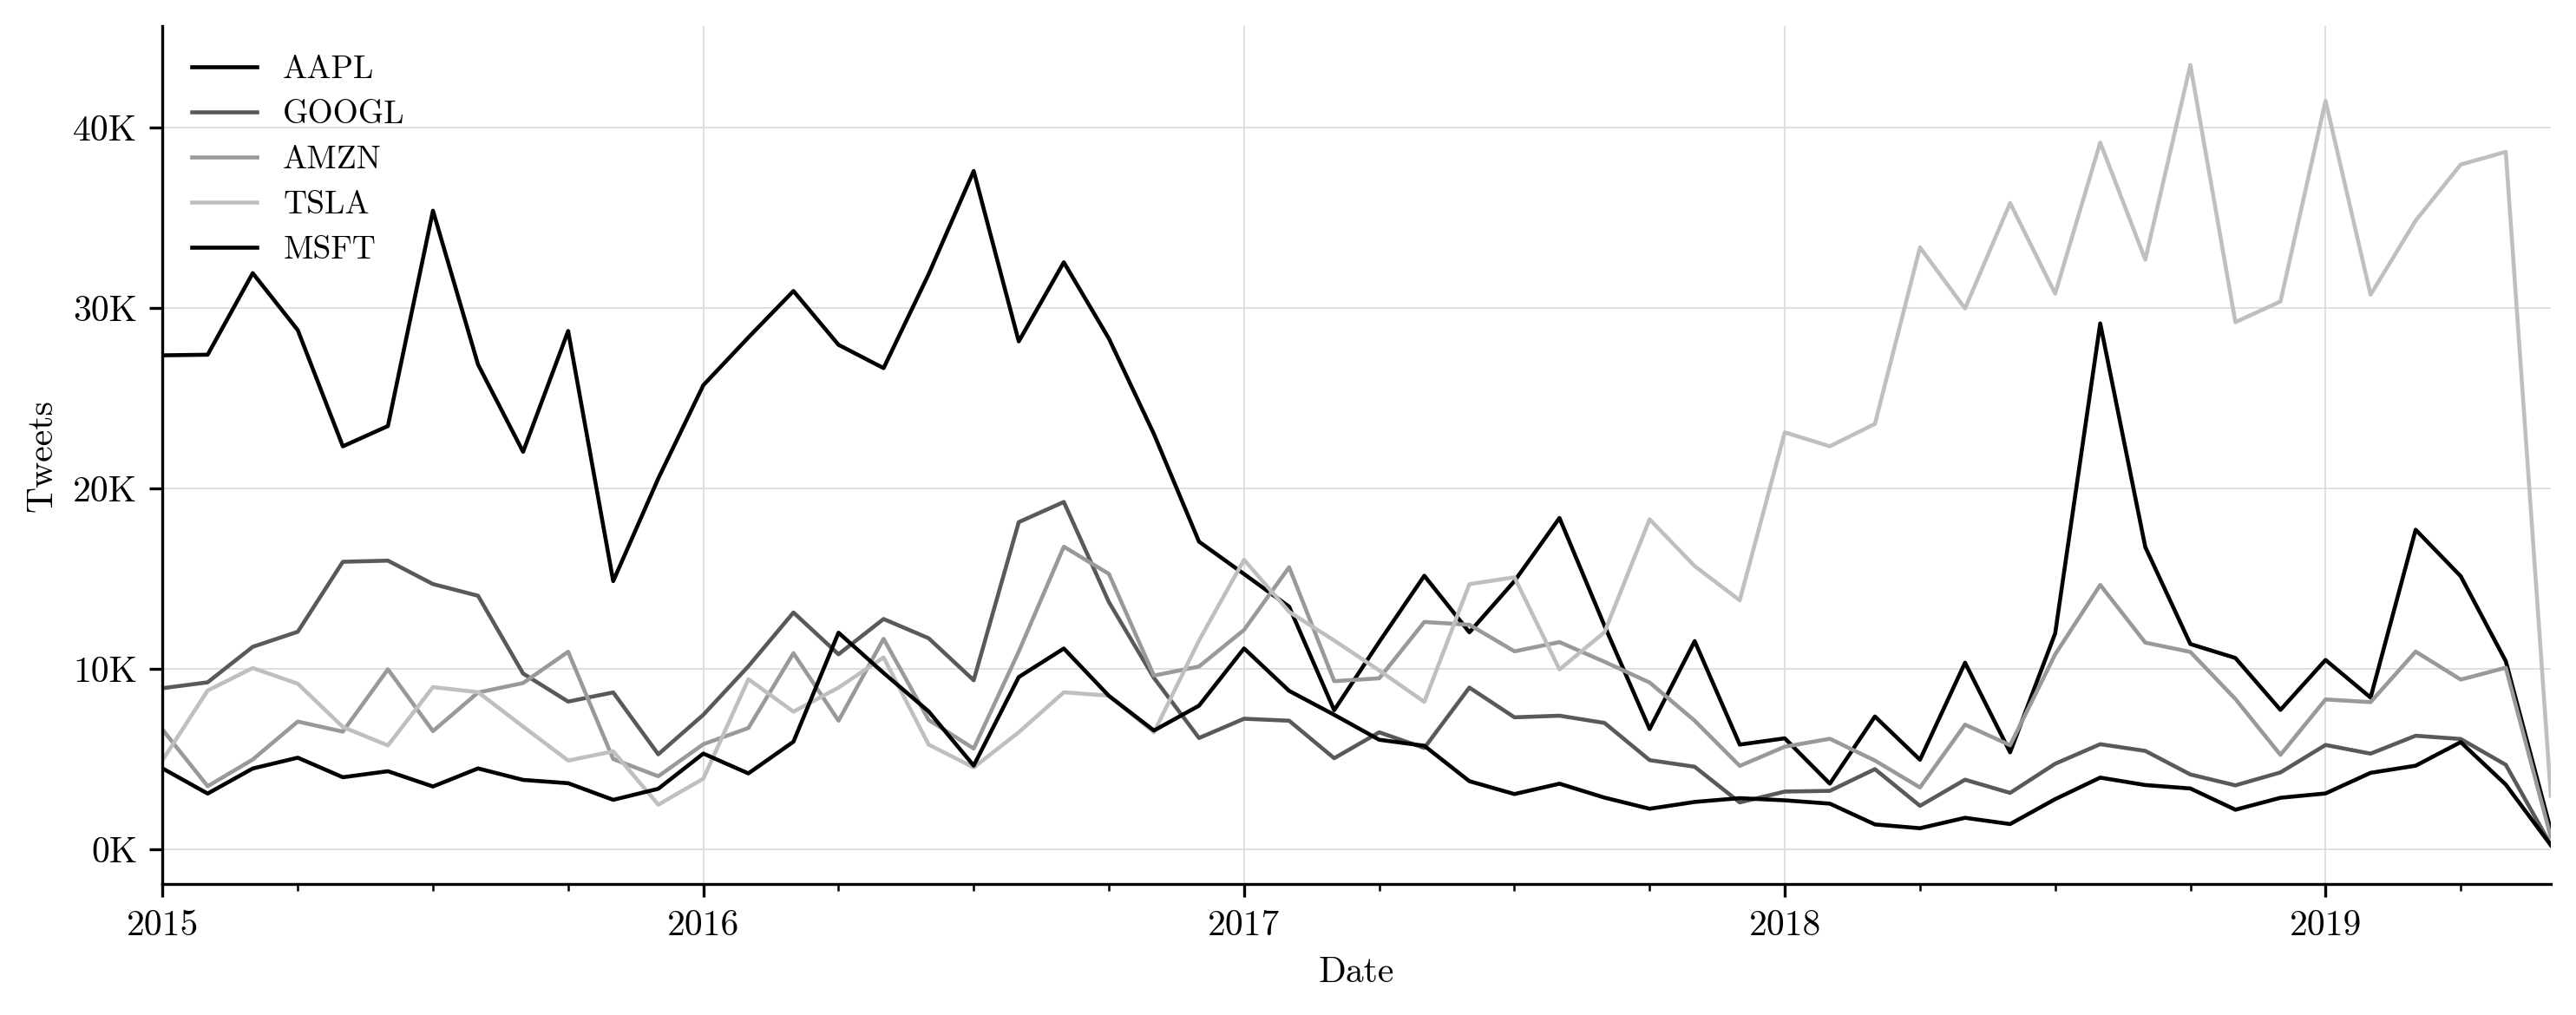
\includegraphics[width=0.8\textwidth]{media/tweets_per_period.png}
\end{figure}


\begin{figure}[h!]
\centering
\caption{Average tweets count per day, week and administrative quarter}
\label{fig:tweets_per_period}
\begin{minipage}{0.8\textwidth}
    \centering
    \textit{Daily}
    \vspace{0.1em}
    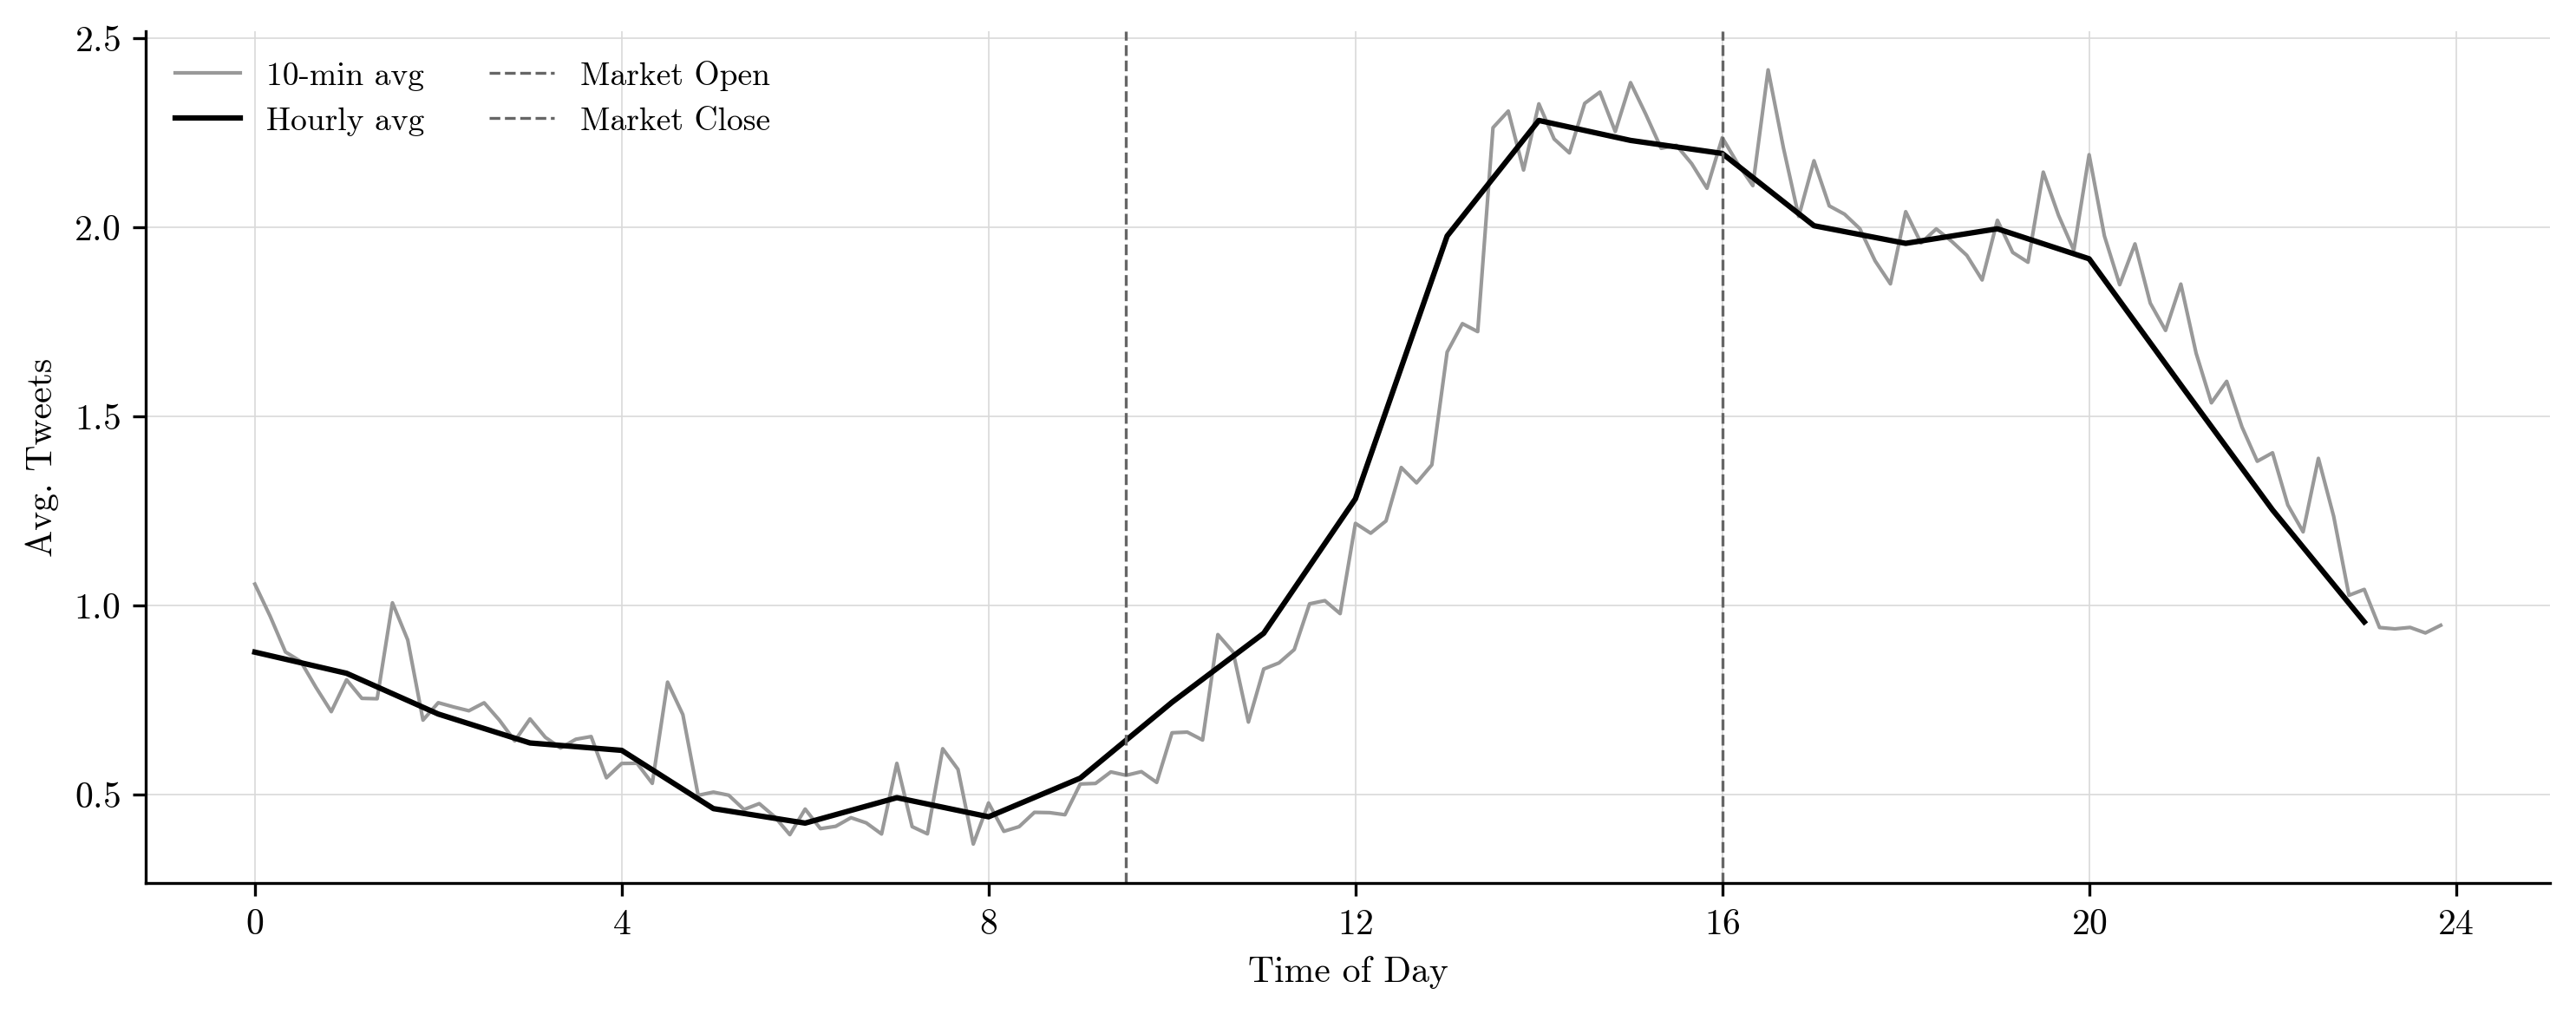
\includegraphics[width=\linewidth]{media/tweets_daily.png}
\end{minipage}
\vspace{1em}

\begin{minipage}{0.8\textwidth}
    \centering
    \textit{Weekly}
    \vspace{0.1em}
    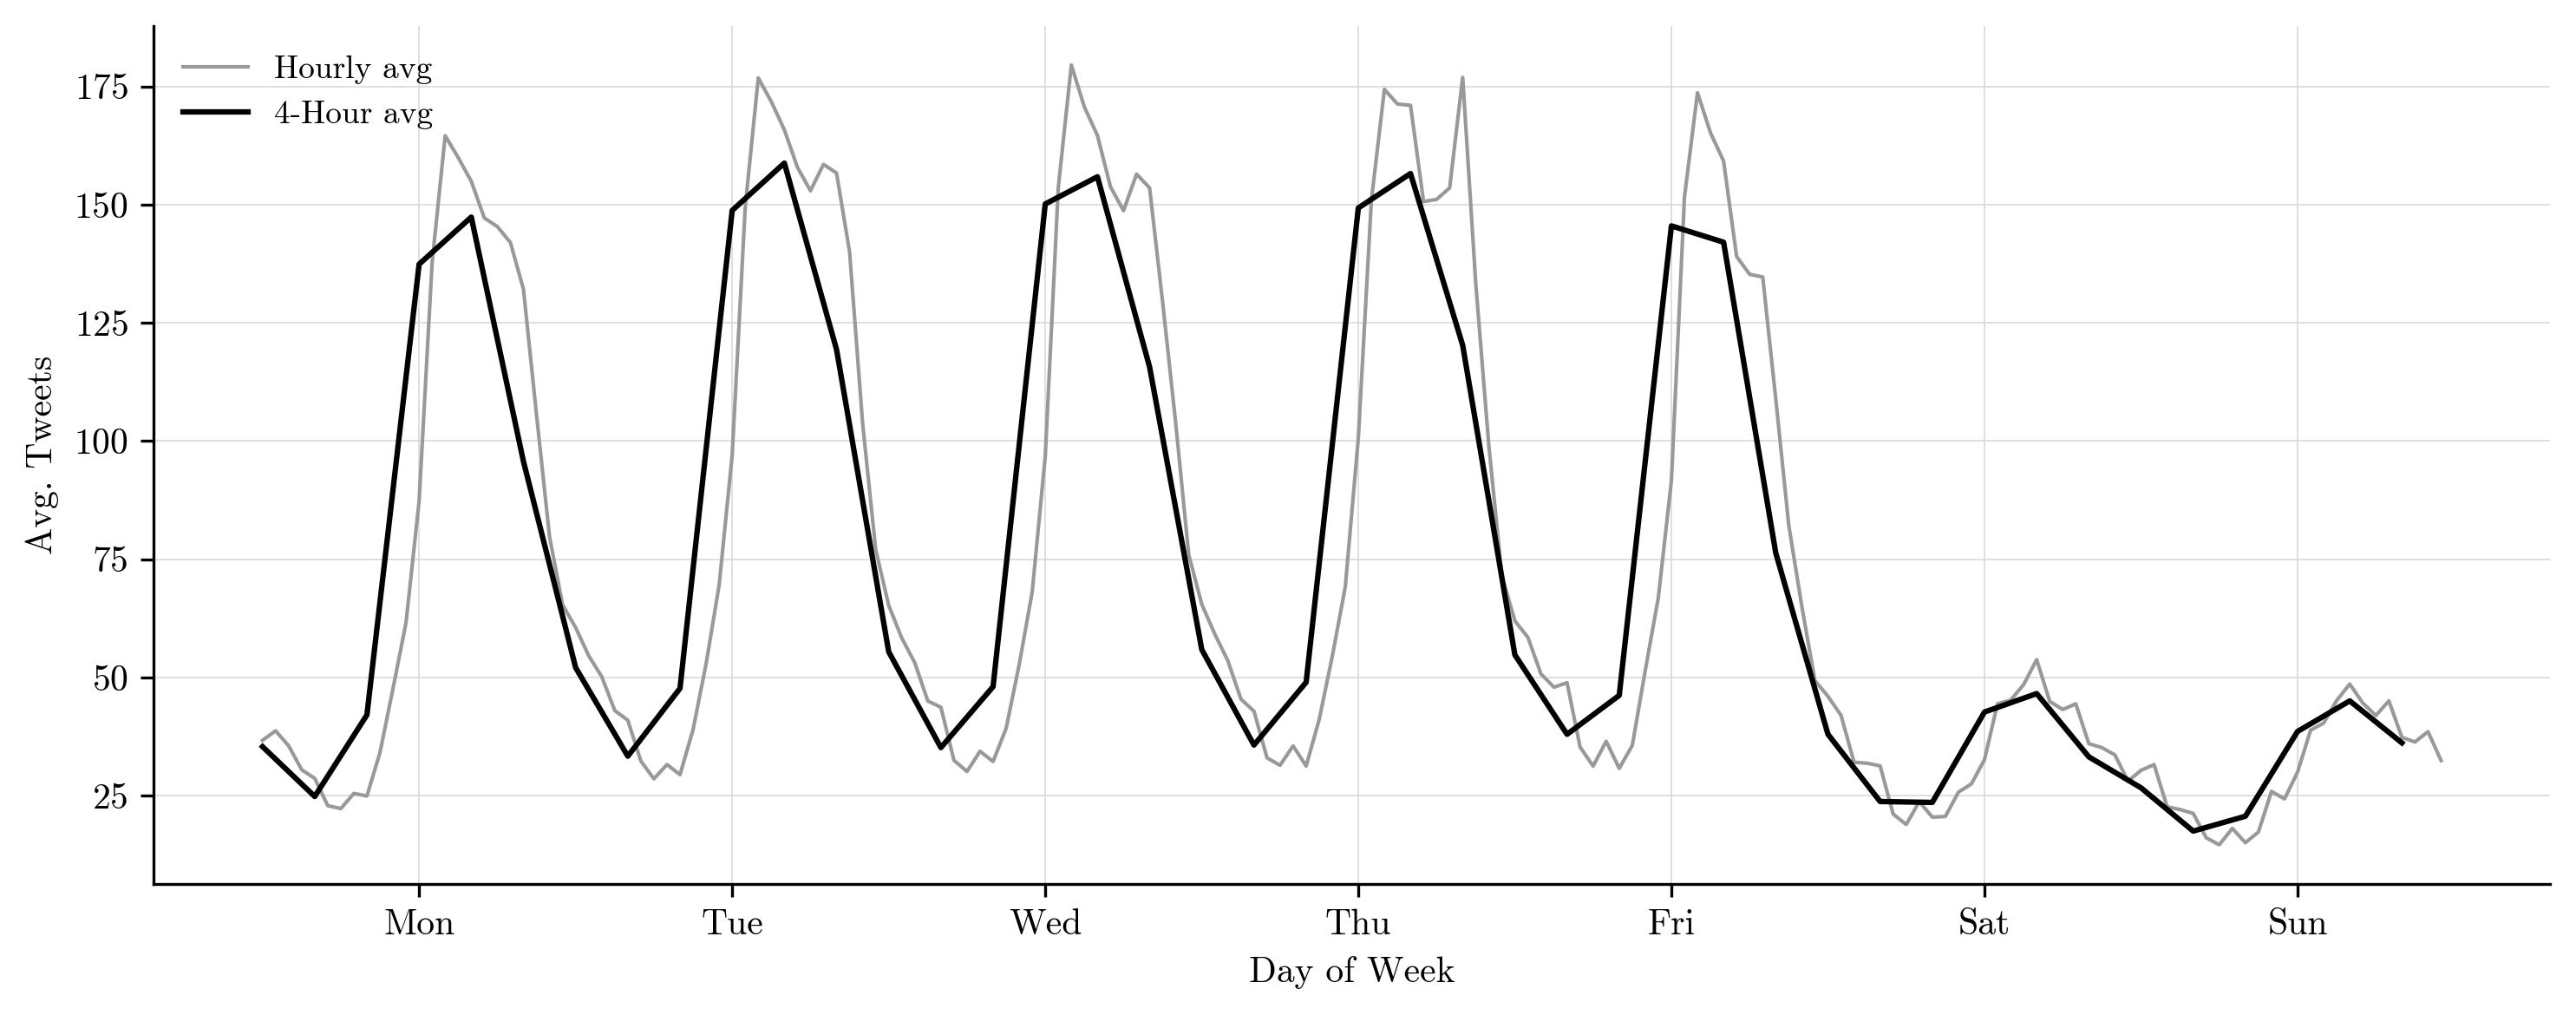
\includegraphics[width=\linewidth]{media/tweets_weekly.png}
\end{minipage}
\vspace{1em}

\begin{minipage}{0.8\textwidth}
    \centering
    \textit{Quarterly}
    \vspace{0.1em}
    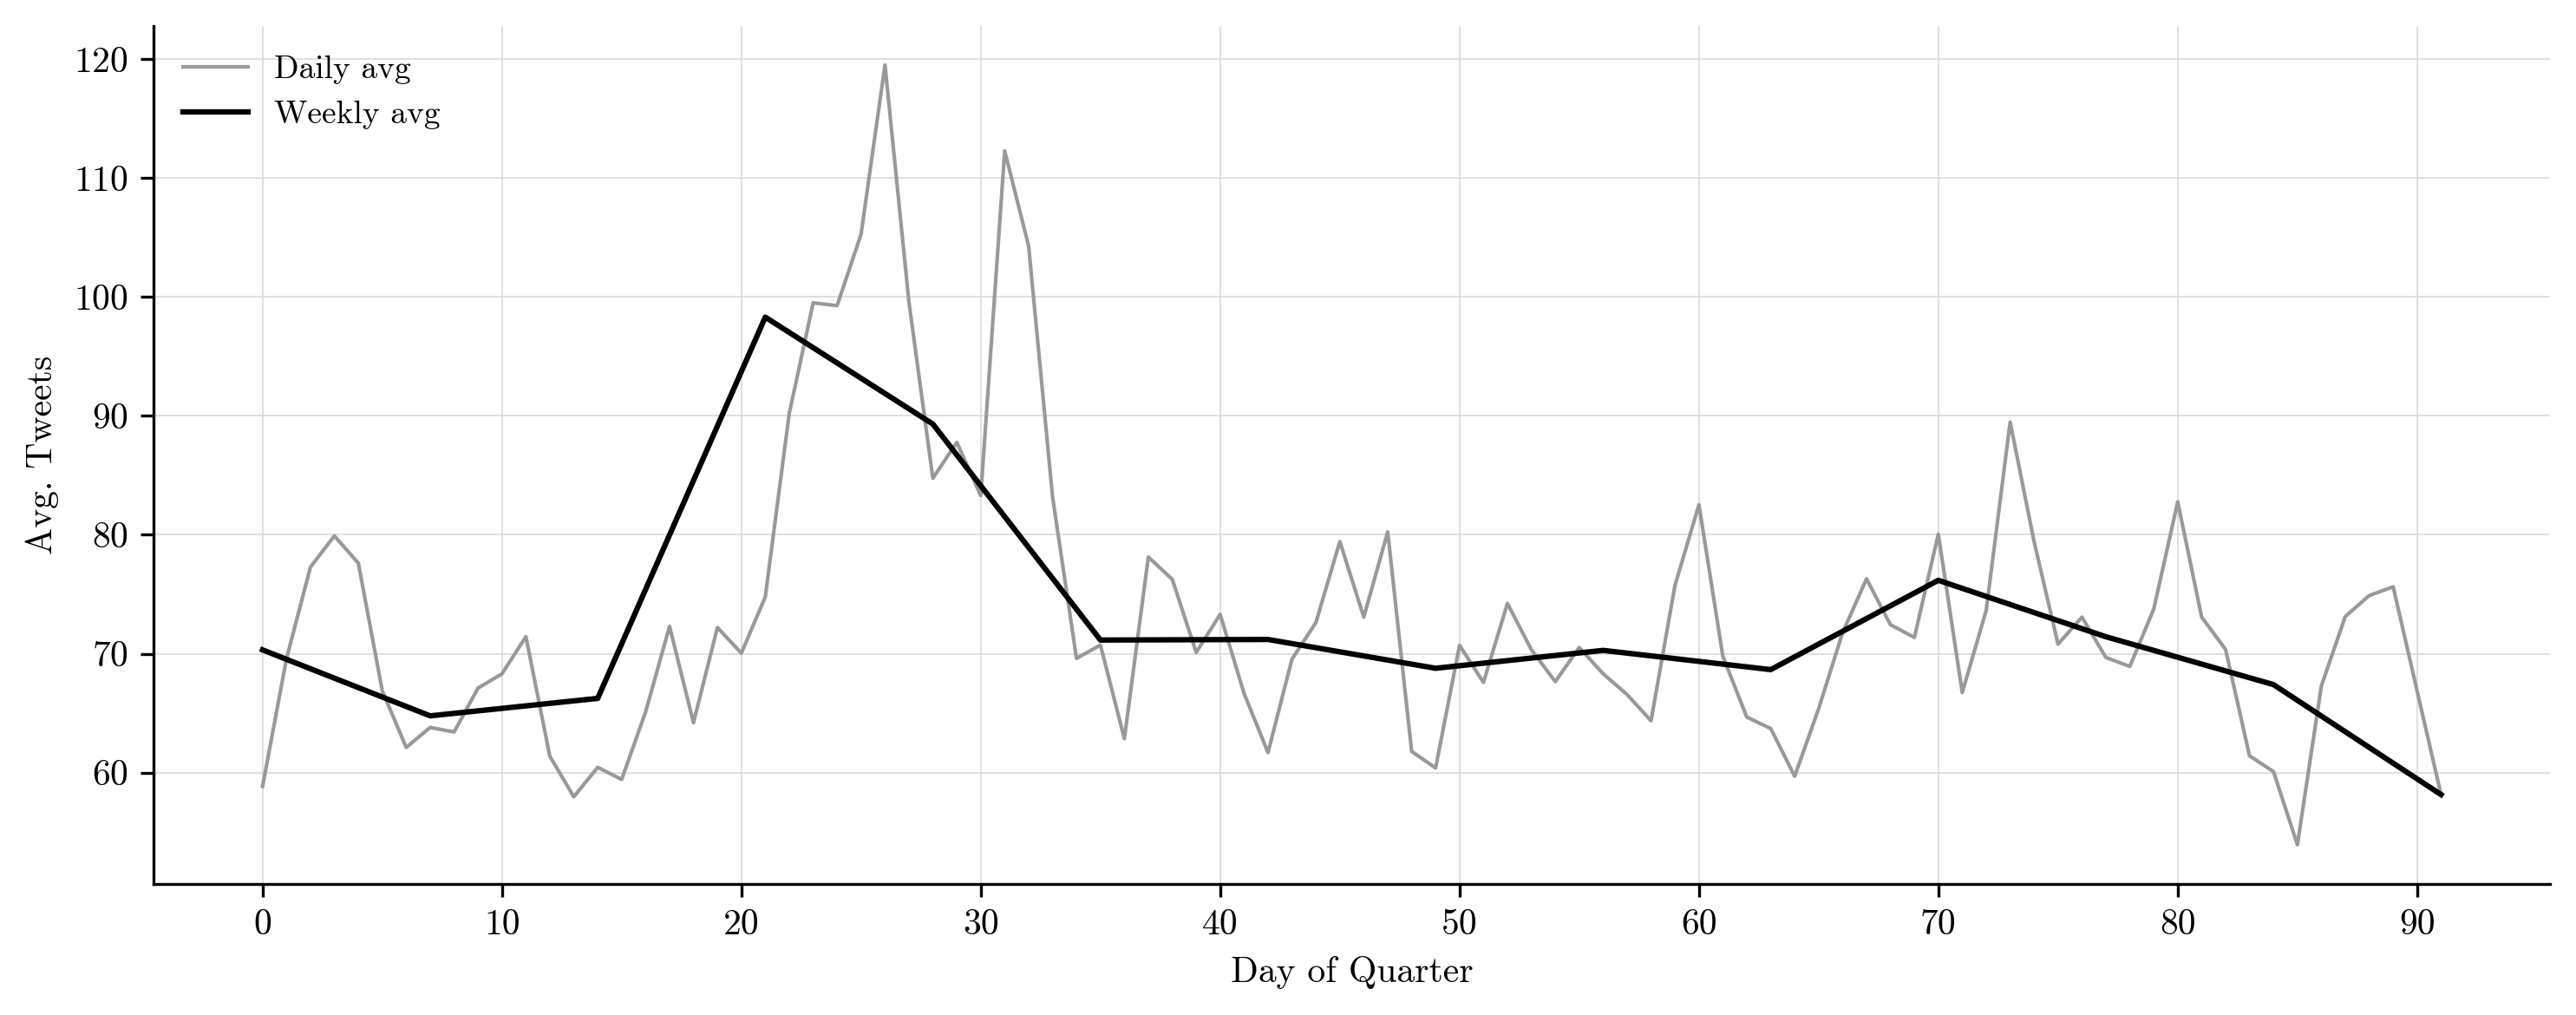
\includegraphics[width=\linewidth]{media/tweets_quarterly.png}
\end{minipage}
\end{figure}


\subsection{Headlines}
Following current sentiment analysis literature \autocite{gite2021explainable,shao2025revisiting}, we add newspaper headlines to our analysis, as a reflection of aggregated institutional beliefs. We scrape firm pages on the Financial Times, fetching headline and date of the article. After cleaning, only 3,898 out of 8,308 articles remain usable for our period\footnote{Many articles are wrongly categorized.}. Hence, we also scrape Reuters, The Guardian, Bloomberg, The New York Times, The Wall Street Journal, CNBC and BBC\footnote{We made the choice not to use Yahoo Finance. Despite providing market-oriented news only, the quality of certain sources are questionable, often more oriented towards sensational news for day traders, not matching institutional quality.}. Instead of designing advanced scrapers to counter individual security norms, we leverage Google search engine with the query \texttt{intitle:{keyword} site:www.{site}.com after:2014-12-31 before:2020-01-01}. We use firm name, products names and CEO names as keywords\footnote{We use the following keywords for each firm. AAPL: Apple, Iphone, Steve Jobs, Tim Cook, iPad, AirPods, MacBook; AMZN: Amazon, Jeff Bezos, AWS; GOOG/GOOGL: Google, Sundar Pichai, Alphabet; MSFT: Satya Nadella, Microsoft; TSLA: Tesla, Model 3, Elon Musk.}. The main limitation of this method is that headlines are sometimes truncated in Google results. After cleaning our results(foreign languages, wrong thematic, customer-oriented articles, guides\footnote{We remove all articles mentioning apples (fruit), the Amazon(forest), and consumer-oriented articles identified using keywords such as "How...", "review", "games", "which", "tips", "tricks", "best", "app", "guide", "opinion", "What...", "Why...", "How...", etc.}), we obtain a total of 11532 headlines.   \\

\subsection{Financial metrics}
For financial metrics, we obtain historical prices for the period from the dataset provided and use the closing price, adjusted returns, adjusted returns over the previous three days and seven days, as well as standard deviation of adjusted closing prices over the past 20 days rolling window. We also use global financial metrics obtained through \href{https://fred.stlouisfed.org/categories/46}{FRED}, including S\&P 500 daily volume and returns, as well as VIX price. We decided not to use daily stock volume as they were highly correlated to S\&P 500 volume. We also do not use risk-free rate, since its slow evolution does not match the short horizon of our forecassting targets. We use return from $d+1$ market open to $d+1$ market close as the one day target. For the seven days target, we compute returns from $d+1$ market open to $d+7$ market close. \\

\section{Sentiment Analysis}

Following \textcite{shao2025revisiting}, we compute sentiment scores for our textual data (tweets and headlines) using a progression of methods of increasing complexity, from lexicon-based approaches to pre-trained language models. \\

We begin with two lexicon-based methods. For VADER, the final score is obtained by subtracting the negative sentiment score from the positive sentiment score of each input. For Bag of Words (BoW), we compute:

 $$\text{BoW score}=
\begin{cases}
\frac{\text{count}_p-\text{count}_n}{\text{count}_p+\text{count}_n}, & \text{if count}_p + \text{count}_n > 0 ;\\
0, & \text{otherwise} ;
\end{cases}
$$

where $\text{count}_p$ and $\text{count}_n$ denote the count of positive and negative words, respectively. The NLTK opinion lexicon underlying this approach offers limited coverage of financial vocabulary; although we manually extend it with domain-specific positive and negative terms, it still produces discrete sentiment scores (-1,0,1) for most tweets. We complement these two methods with TextBlob, which directly returns a continuous polarity score in [-1,1]. \\

We then turn to LLMs, which are considerably more resource-intensive but better suited to noisy, informal text. We first use FinBERT, a BERT-based model further pre-trained on financial corpora. Running FinBERT through HuggingFace on our 3 million tweets took over 15 hours, against a few seconds to a few minutes for each of the lexicon-based methods above. We also evaluate a pre-trained RoBERTa model fine-tuned for sentiment analysis, accessed through HuggingFace. Following \textcite{shao2025revisiting}, we find that while FinBERT performs well on structured, formal financial text such as bank statements and analyst reports, it is less effective on noisy, large-scale social media data. Given the informal and heterogeneous nature of our tweet corpus, we retain RoBERTa as our preferred LLM-based sentiment measure for the remainder of the analysis. This computation again took over 15 hours. \\

We then aggregate sentiment scores over distinct time windows. \textcite{shao2025revisiting} rely on daily sentiment (00:00 to 23:59). We experiment with this same daily window, but also with windows aligned with market activity. Under the assumption that overnight sentiment, not yet priced in, carries predictive power, we aggregate sentiment over the window spanning market close on day $d$ to market open on day $d+1$. We additionally experiment with a second 24-hour window, this time spanning market open on day $d$ to market open on day $d+1$. Both windows avoid look-ahead bias, since our prediction targets are computed from market open on day $d+1$ onward, never from market close on day $d$. \\

For each of these windows, an average sentiment score must be computed. \textcite{shao2025revisiting} weight tweets by follower count; lacking equivalent follower-level data, we instead rely on three alternative weighting schemes:
$$\begin{aligned}
&\text{General Avg}_z=\frac{1}{T}\sum^T_{i=1}S_{i,z} \\
&\text{Tweet Influential Weight}_z=\frac{\sum^T_{i=1}(D_i+1)\times S_{i,z}}{\sum^T_{i=1}(D_i+1)} \\
&\text{Tweet Log-Weighted}_z=\frac{\sum^T{_i=1}\log(1+\text{comments}_i+\text{RT}_i+\text{likes}_i)\times S{i,z}}{\sum^T_{i=1}\log(1+\text{comments}_i+\text{RT}_i+\text{likes}_i)}\
\end{aligned}$$
We compare the performance of a model using a simple unweighted average, a model weighting tweets by an influential flag $D_i$ (set to 1 if any of a tweet's engagement metrics falls within the 99th percentile of our dataset), and a model using a simple log-weighted average based on each tweet's engagement metrics. As headlines lack equivalent engagement metrics, we use a simple unweighted average over the window for news sentiment. After experimentation with our models, we find that the overnight window and the standard daily window perform best, while log-weighting yields the best results among the three averaging schemes. \\

\autoref{fig:finbert_sentiment} shows the daily average FinBERT sentiment for AAPL and TSLA\footnote{Mapping: a tweet labeled positive is assigned $+1$, negative $-1$, and neutral $0$.}. Note that FinBERT is not retained for the remainder of the analysis.

\begin{figure}[h!]
\centering
\caption{Daily average FinBERT sentiment}
\label{fig:finbert_sentiment}
\begin{minipage}{0.8\textwidth}
    \centering
    \textit{\$AAPL}
    \vspace{0.1em}
    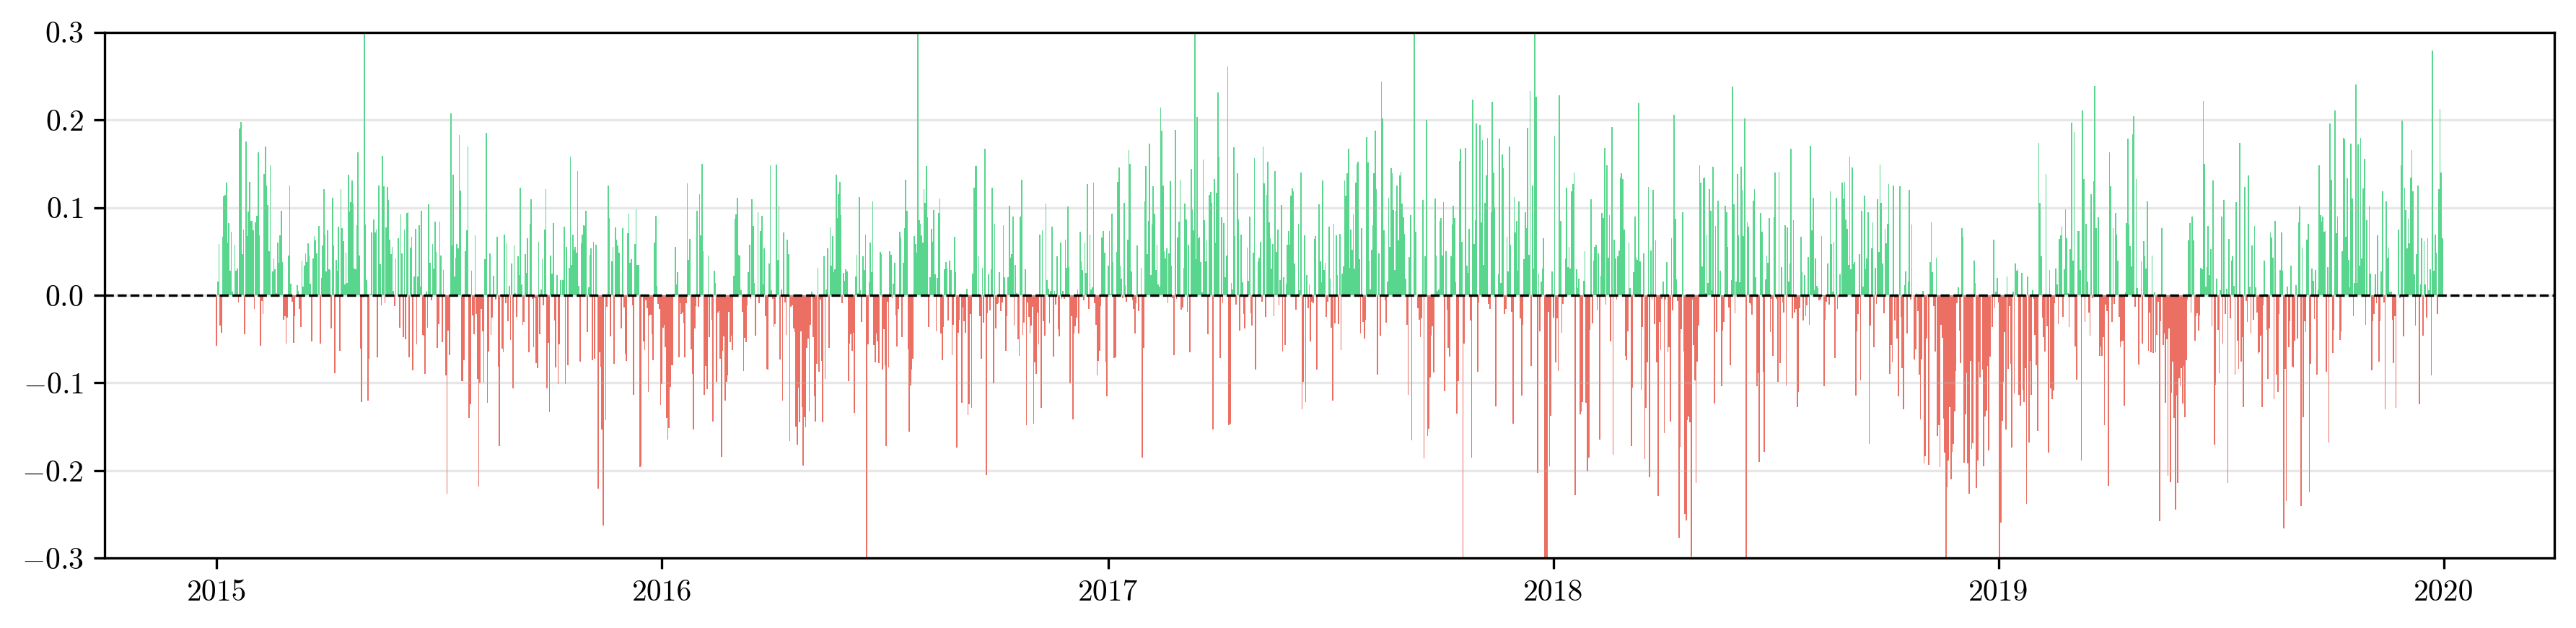
\includegraphics[width=\linewidth]{media/sentiment_AAPL.png}
\end{minipage}
\vspace{1em}

\begin{minipage}{0.8\textwidth}
    \centering
    \textit{\$TSLA}
    \vspace{0.1em}
    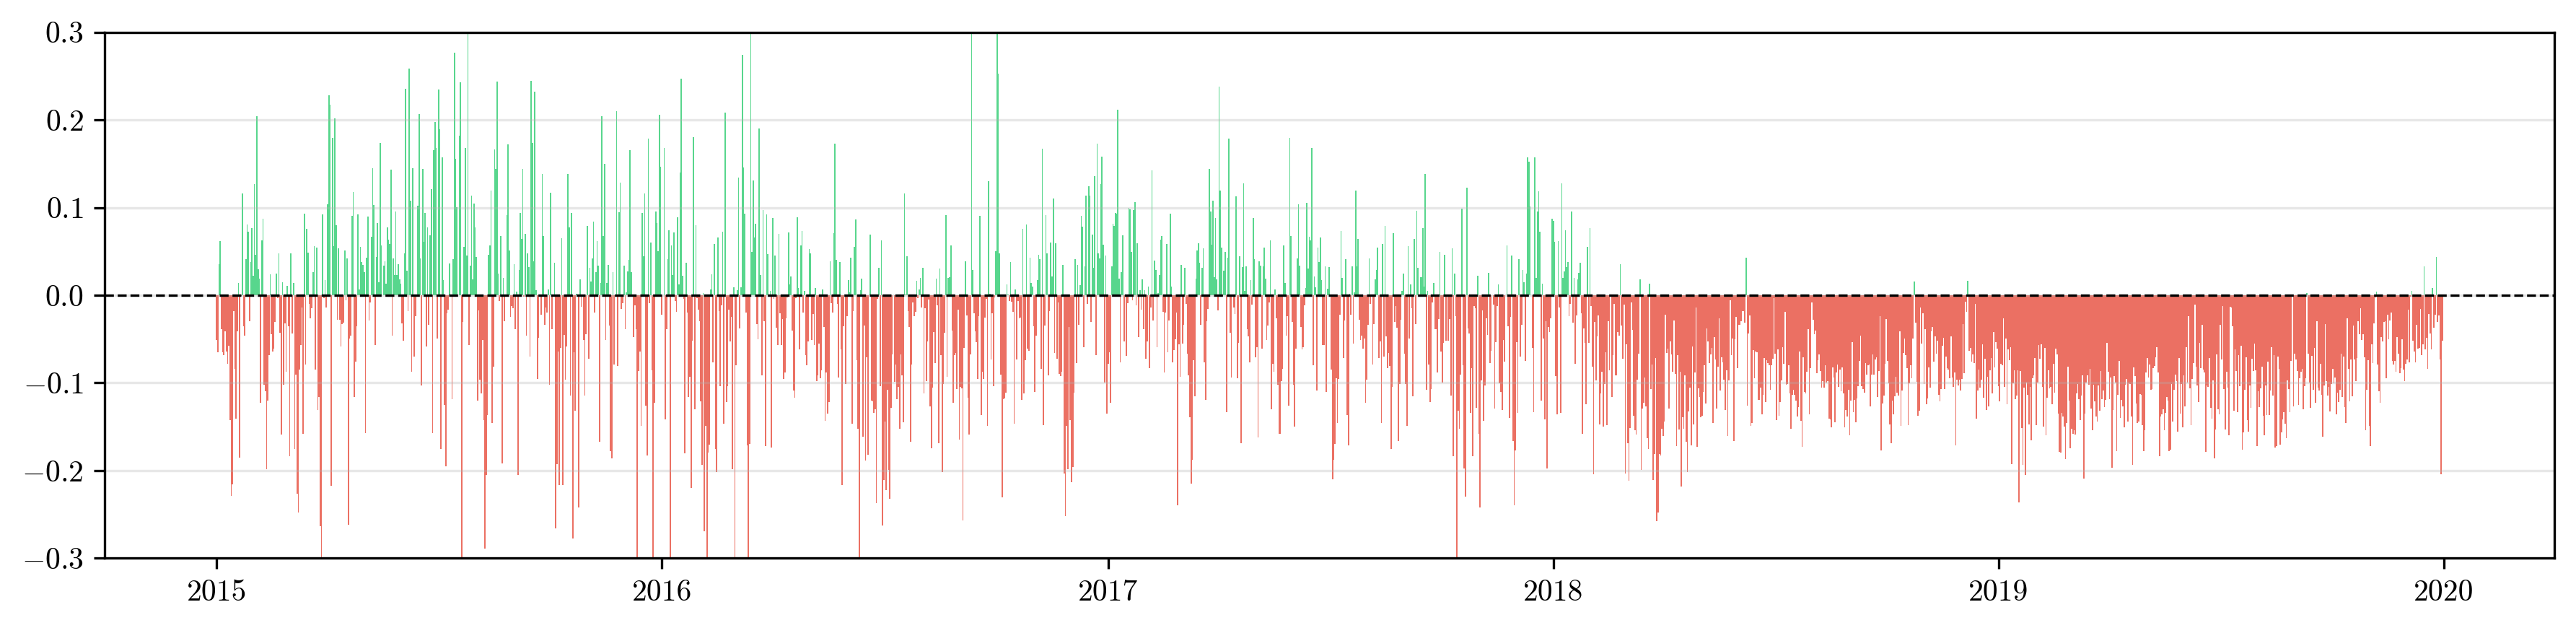
\includegraphics[width=\linewidth]{media/sentiment_TSLA.png}
\end{minipage}
\end{figure}


Headline sentiment suffers from substantial missingness, ranging from 14.8\% of days without headlines for AAPL to 54.8\% for Microsoft. To address this, we experiment with several approaches to filling missing values. After iterating across our models, an Exponentially Weighted Moving Average (EWMA) over a 5-day window with a decay factor of 0.5 was selected. \\

At the global level, we observe moderate correlation across our different sentiment measures, suggesting minor differences but no major disagreement (\autoref{fig:corr_heatmap}).

\begin{figure}[h!]
\centering
\caption{Global sentiment correlation matrix}
\label{fig:corr_heatmap}
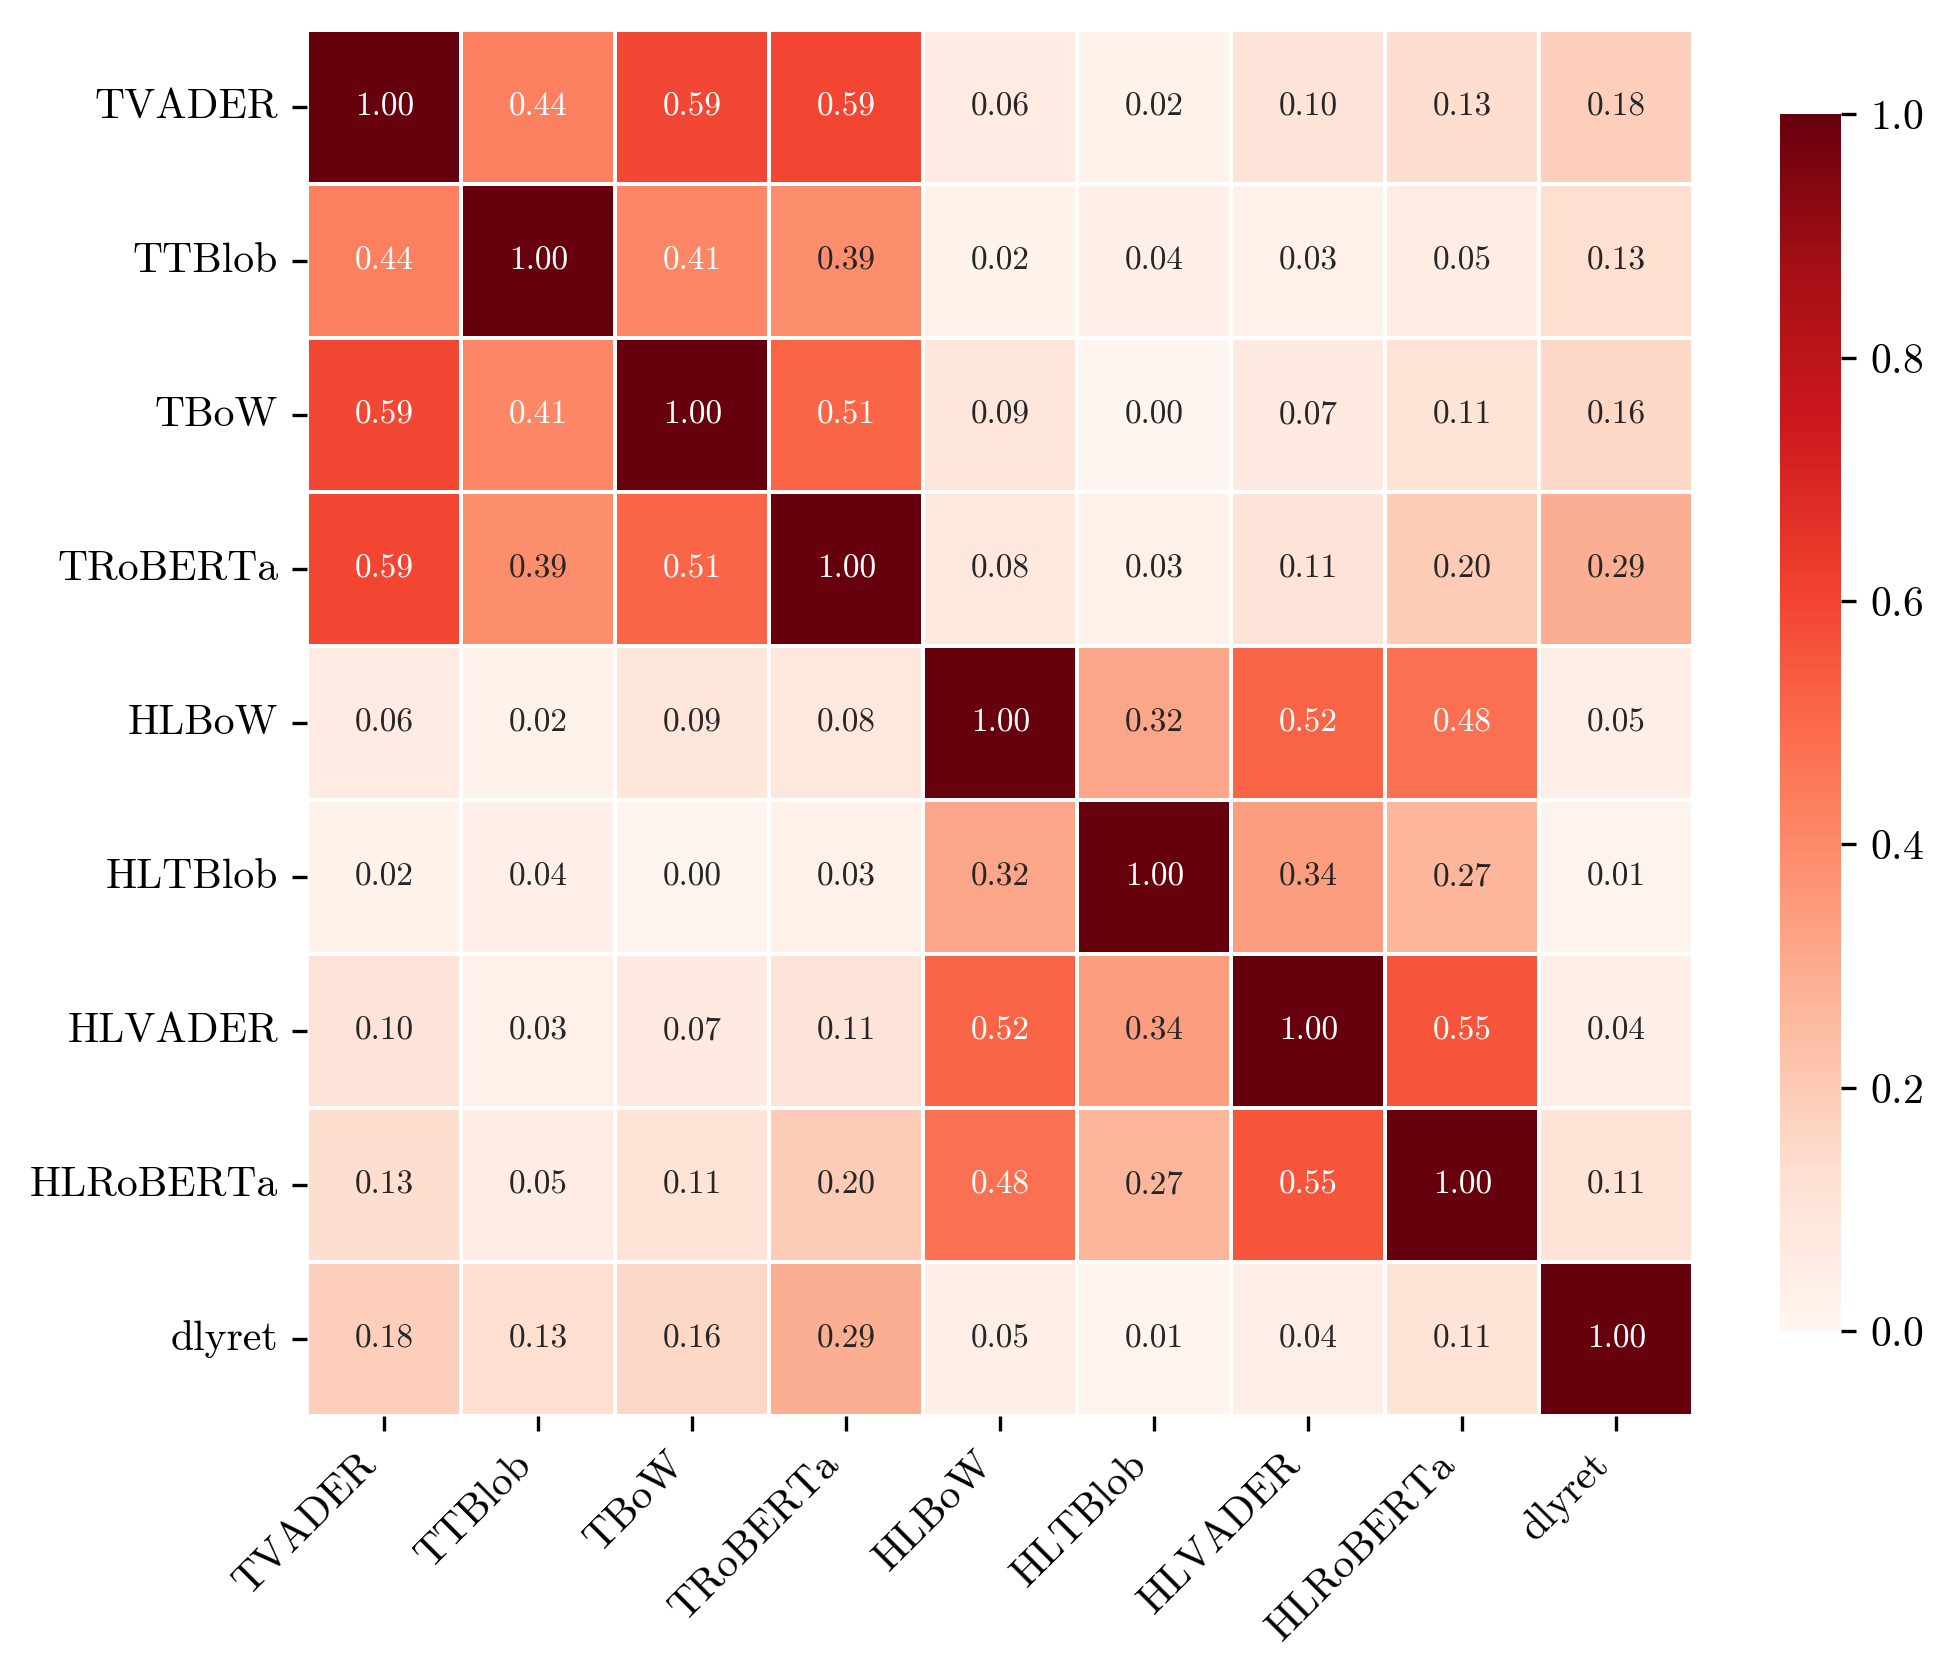
\includegraphics[width=0.5\textwidth]{media/corr_heatmap.png}
\end{figure}



\subsection{HD-SURDLM and benchmarks}

Following \textcite{shao2025revisiting}, our core model is the Heterogeneous Dynamic Seemingly Unrelated Regression with Dynamic Linear Models (HD-SURDLM), a Bayesian state-space framework that jointly models multiple assets through stock-specific intercepts, time-varying sentiment and financial coefficients, and a cross-sectional error covariance structure capturing spillover effects between stocks. Parameters are estimated via Gibbs sampling, using a stabilized Filter Forward Backward Sampling (FFBS) step that improves numerical convergence relative to standard implementations. \\

We run a lighter version of the model on half of our sample, with 2,000 iterations and a 500-iterations burn-in instead of 5,000 and 1,000 respectively, targeting $d+1$ returns (\textit{ret1}). We forward-fill the few missing tweet sentiments. We grid-search over all individual tweet sentiment combinations (15), all headline sentiment combinations (15), all combined tweet-headline combinations ($15 \times 15$), and the three averaging schemes aforementioned, totaling 1,669 runs. We further vary the sentiment window (overnight vs. daily), the noise-to-signal ratio $\delta$, and the sentiment input horizon (same-day sentiment vs. multi-day EWMA-smoothed sentiment with varying decay factors).  The log-weighted average on tweet metrics performs better, and models using overnight features represent seven out of the ten best performing models. Best models most often use VADER and BoW analysis, while RoBERTa is never among the top performers. Both Tweets only, headlines only and mixed models perform good, but models using only tweets represent 8 out of the 10 best performing configurations for returns $d+1$. Based on shortlisted \textit{ret1} configurations, we run an additional 720 configurations for the 7-day horizon (\textit{ret7}).For $ret7$, best configurations often use solely headlines (6 out of the top 10), with no model based only on tweets.  \\

As benchmarks, we use an always-up baseline, Random Forest, Lasso, SVR, MLP, RNN, LSTM, and a hybrid CNN-LSTM, each evaluated both as a binary classifier and as a continuous regressor. We use a 80/20 split both for our HD-SURDLM model and our benchmarks.\\


\section{Results}

\subsection{Models comparison}
Here are the results after running the HD-SURDLM on 5,000 iterations and 1,000 iterations burn-in on the full sample. For the $ret1$ target, we select the best model, using only financial features and tweeter sentiment extracted via VADER. We leverage the confidence given by our bayesian model and base our results only on predictions that have a standard prediction of under 0.002, which reprents 70\% of the sample. \autoref{tab:model_performance1} underlines that our model consistently outperforms benchmark models, but doesn't outperform the basic up model on recall and F1 score, except on hit-rate. This seems to indicate difficult fit and poor explanatory power over the sample. \\

\begin{table}[h]
\centering
\caption{Mean 1-day horizon metrics across models (T=VADER, $\delta=0.9$) (\%)}
\label{tab:model_performance1}
\setlength{\tabcolsep}{5pt}
\begin{tabular}{lcccccccccccccccc}
\toprule
Metric & 
\rotatebox{90}{Up} & 
\rotatebox{90}{RndFor\_r} & 
\rotatebox{90}{RndFor\_c} & 
\rotatebox{90}{Lasso\_r} & 
\rotatebox{90}{Lasso\_c} & 
\rotatebox{90}{SVR\_c} & 
\rotatebox{90}{MLP\_r} & 
\rotatebox{90}{MLP\_c} & 
\rotatebox{90}{RNN\_r} & 
\rotatebox{90}{RNN\_c} & 
\rotatebox{90}{LSTM-REG\_r} & 
\rotatebox{90}{CNN-LSTM\_r} &
\rotatebox{90}{HD-SURDLM} \\
\midrule
\textbf{H-R}  & 51.7 & 49.5 & 48.6 & \textbf{53.6} & 51.9  & 48.9 & 48.5 & 49.7 & 52.4 & 50.3 & 51.0 & 52.0 & \underline{53.1} \\
\textbf{Pre.} & 51.7 & 52.9 & 51.8 & 46.0 & 44.6 & 52.4 & 52.4 & 52.5 & 55.4 & \textbf{55.5} & 53.1 & 52.3 &  \underline{54.7} \\
\textbf{Rec.}    & \textbf{100.0} & 48.3 & 48.4 & 66.9 & \underline{71.8} & 54.0 & 49.0 & 58.3 & 54.3 & 38.4 & 60.7 & 61.3 & 69.5 \\
\textbf{F1}        & \textbf{68.1} & 50.5 & 50.0 & 54.0 & 54.4 & 52.5 & 50.5 & 54.9 & 54.8 & 44.2 & 56.2  & 54.1  & \underline{61.2} \\
\bottomrule
\end{tabular}
\end{table}

For the $ret7$ target, we once again use our best model, that relies on financial metrics and headline sentiment measured using the Bag of Words approach. Instead of using daily sentiment, we feed the model with average sentiment over the past eight days. The noise-to-signal ratio is this time set at 0.98 instead of the 0.9 used by \textcite{shao2025revisiting}. Using the 0.002 standard deviation threshold is impossible since only three observations fall under this threshold; we hence consider the entire sample. Once again, our model outperforms basic machine learning models, but is tied with the basic up-only model. \\


\begin{table}[h]
\centering
\caption{Mean 7-day horizon metrics across models (HL=BoW, AVG=8, $\delta=0.98$) (\%)}
\label{tab:model_performance2}
\setlength{\tabcolsep}{5pt}
\begin{tabular}{lccccccccccccc}
\toprule
Metric & 
\rotatebox{90}{Up} & 
\rotatebox{90}{RndFor\_r} & 
\rotatebox{90}{RndFor\_c} & 
\rotatebox{90}{Lasso\_r} & 
\rotatebox{90}{Lasso\_c} & 
\rotatebox{90}{SVR\_c} & 
\rotatebox{90}{MLP\_r} & 
\rotatebox{90}{MLP\_c} & 
\rotatebox{90}{RNN\_r} & 
\rotatebox{90}{RNN\_c} & 
\rotatebox{90}{LSTM-REG\_r} & 
\rotatebox{90}{CNN-LSTM\_r} & 
\rotatebox{90}{HD-SURDLM} \\
\midrule
\textbf{H-R}  & \underline{58.2} & 50.9 & 48.2 & 53.2 & 51.7 & 48.3 & 49.0 & 50.4 & 50.2 & 48.7 & 52.1 & 50.6 & \textbf{58.3} \\
\textbf{Pre.} & \underline{58.2} & 54.7 & 51.7 & 45.5 & 52.7 & 51.8 & 52.6 & 53.2 & 53.1 & 55.2 & 54.8 & 52.7 & \textbf{64.6} \\
\textbf{Rec.}  & \textbf{100.0} & 48.2 & 45.6 & 69.3 & 55.2 & 50.6 & 49.1 & 58.2 & 55.9 & 29.1 & 56.4 & 55.6 & \underline{78.3} \\
\textbf{F1}   & \textbf{73.6} & 51.2 & 48.4 & 54.4 & 49.8 & 50.6 & 50.7 & 55.1 & 54.4 & 36.6 & 55.2 & 52.0 & \underline{70.5} \\
\bottomrule
\end{tabular}
\end{table}

Our results seem to underline that our model doesn't find a real edge in the market sentiment we extracted, only reflecting the upward market trend of the sample period.

\subsection{Market simulation}
We still simulate trading results using our model on out-of-sample data. Following the instructions, we design a simple long-only, no risk-management nor position sizing backtesting framework, fully reinvesting the remaining initial capital (starting at \$10,000) in each position, with no overlapping positions. For $ret1$, we only use days where the predicted standard deviation is under 0.002. For $ret7$, we use all our predictions, but add a seven days cooldown after each trade to avoid position overlap that would not match the \$10,000 capital restriction. We consider a 3\% simplified risk free rate and 252 trading days.\\

\begin{table}[h]
\centering
\caption{Market simulation results (long-only, \$10,000 seed capital)}
\label{tab:backtest_results}
\renewcommand{\arraystretch}{1.2}
\setlength{\tabcolsep}{8pt}
\begin{tabular}{lccc}
\toprule
Metric & $ret1$ & $ret7$ & Buy\&Hold\\
\midrule
Trades              & 227          & 52           & $-$ \\
Final Capital (\$)  & 15{,}144.87  & 18{,}055.40  & 12{,}868.96\\
Total Return (\%)   & 51.45        & 80.55        & 28.69\\
Win Rate (\%)       & 56.39        & 61.54        & $-$ \\
Max Drawdown (\%)   & $-$8.44      & $-$17.42     & $-$6.14 \\
Sharpe Ratio        & 2.5534       & 2.0637       & 1.7244 \\
Profit Factor       & 1.5673       & 2.4482       & $-$ \\
\bottomrule
\end{tabular}
\end{table}

Logically, we notice more trades for the daily strategy than for the weekly one, as expected with the implemented cooldown. Both strategies are profitable, which is reassuring given the 28.69\% equally-weighted buy and hold returns. Our strategies still achieve a higher Sharpe Ratio, indicating some improvement over the buy and hold model. 


\section{Conclusion}

Overall, our results echo the central finding of \textcite{shao2025revisiting}: while the HD-SURDLM model consistently outperforms standard machine learning and deep learning benchmarks across both the one-day and seven-day horizons, it fails to meaningfully outperform a naive always-up baseline on recall and F1 score. This suggests that, despite the richness of our textual and financial feature set, the model struggles to extract a genuine predictive edge from sentiment during a period largely characterized by a sustained bull market, where simply betting on continued upward movement proves difficult to beat. \\

Our market simulation nonetheless offers a more encouraging perspective: both the $ret1$ and $ret7$ trading strategies generate higher risk-adjusted returns than an equally-weighted buy-and-hold portfolio, achieving Sharpe ratios of 2.55 and 2.06 respectively, against 1.72 for the benchmark. This indicates that, even in the absence of a clear statistical edge on classification metrics, the model's confidence-filtered predictions may still carry some economic value when translated into trading decisions. \\

Several limitations remain. Headline sentiment coverage is uneven across firms, with up to 54.8\% of days missing news data for Microsoft, which may bias our EWMA-based imputation. Additionally, the absence of follower-level engagement data forced us to rely on alternative weighting schemes that may not fully capture tweet influence as intended by \textcite{shao2025revisiting}. Future work could extend this analysis to more volatile market regimes, further explore FinBERT's underperformance on social media data, and investigate whether the Granger-causal relationships identified in earlier literature (e.g., \textcite{bollen2011twitter}) persist once richer financial controls are accounted for.

\printbibliography

\end{setstretch}
\end{document}